\documentclass[aps,prl,twocolumn,superscriptaddress,amsmath,amssymb,10pt]{revtex4-2}
\usepackage{graphicx}
\usepackage{bm}
\usepackage[colorlinks=true,linkcolor=blue,citecolor=blue,urlcolor=blue]{hyperref}

\newcommand{\Lc}{\mathcal{L}}
\newcommand{\J}{\mathcal{J}}
\newcommand{\tr}{\operatorname{tr}}

\begin{document}

\title{Exact energy mode and a dissipative gap transition in the open Sachdev-Ye-Kitaev model}

\author{[Author]}
\affiliation{[Affiliation]}

\date{\today}

\begin{abstract}
We show that the Lindbladian of the Sachdev-Ye-Kitaev (SYK) model with linear Majorana jump operators has an exact eigenoperator for every coupling realization and every $N$: the Hamiltonian itself, $\Lc(H)=-q\mu H$. Because $H$ is simultaneously a left and right eigenvector, it never hybridizes with the rest of the spectrum. The spectral gap is therefore $\Delta=\min\{q\mu,\Gamma_\ast(\mu)\}$, with an exact level crossing and a nonanalytic point $\mu_c$ already at finite $N$. Here $\Gamma_\ast$ is the slowest energy-orthogonal resonance, which stays finite as $\mu\to0$. Combining the large-$N$ Kadanoff-Baym equations with exact diagonalization up to $N=20$, we find $\Gamma_\ast\simeq 2\Gamma_1$, where $\Gamma_1$ is the single-fermion decay rate. This gives $\mu_c\simeq0.32J$ for $q=4$ and $\mu_c=4\J/(q\sqrt{q^2-4})$ at large $q$. Below $\mu_c$ the gap closes linearly and relaxation is controlled by an Ornstein-Uhlenbeck tower of energy modes with rates $kq\mu$. The finite-gap ``anomalous relaxation'' reported for the dissipative SYK model is thus a property of the energy-orthogonal sector only. The same mechanism applies to any Hamiltonian that is homogeneous in the operator-size grading selected by the noise.
\end{abstract}

\maketitle

\emph{Introduction.}---How fast does a strongly chaotic quantum system relax when it is weakly coupled to a Markovian environment? Its Lindbladian spectral gap $\Delta$ sets the asymptotic relaxation rate~\cite{Kessler2012,Minganti2018,Znidaric2015}. For chaotic many-body systems, taking $N\to\infty$ before $\mu\to0$ is expected to leave a \emph{finite} gap in the weak-dissipation limit. This gap is a quantum analogue of Ruelle-Pollicott resonances~\cite{Prosen2002,Mori2024,Jacoby2025,Zhang2026}, and its existence is called anomalous relaxation. The SYK model~\cite{SY1993,Kitaev2015,MS2016} with linear jump operators is the cleanest example. It can be solved at large $N$ through Schwinger-Dyson (SD) equations~\cite{Kulkarni2022,Sa2022,Garcia2023}. Its single-fermion Green's function decays at a rate that stays finite as $\mu\to0$, and the Keldysh contour maps onto a two-site non-Hermitian SYK model with a wormhole-like gravity dual~\cite{Garcia2023,MQ2018}. Exact diagonalization (ED) at small $\mu$, however, shows a gap $4\mu$ that \emph{vanishes} with the dissipation~\cite{Garcia2023}. How these two observations fit together, and what happens at $N=\infty$, has remained unclear~\cite{Garcia2023,Zheng2026}. Mori has argued that conserved quantities generally spoil the singular weak-dissipation limit~\cite{Mori2024}.

Here we resolve this question with an exact statement and a sharp prediction. (i) For any realization of the couplings, any $N$ and any $q$, $H$ is an exact eigenoperator of the Lindbladian with eigenvalue $-q\mu$. Its orthogonal complement is invariant, so the energy mode undergoes an \emph{exact} level crossing with the energy-orthogonal spectrum. (ii) That crossing makes the gap nonanalytic at $\mu_c$, which we determine from the large-$N$ SD equations: $\mu_c\simeq0.323J$ for $q=4$, and $\mu_c=4\J/(q\sqrt{q^2-4})$ for $q\to\infty$. ED shows the same crossing at every finite $N$. (iii) Below $\mu_c$ the gap is $q\mu$, and slow dynamics is governed by an Ornstein-Uhlenbeck (OU) tower of energy modes. A thermal initial state heats quasistatically, $E(t)=E_0e^{-q\mu t}$ exactly, while the energy-orthogonal sector relaxes at the finite rate $\Gamma_\ast$.

\emph{Model.}---We consider $N$ Majorana fermions, $\{\psi_i,\psi_j\}=\delta_{ij}$, with
\begin{equation}
H=\sum_{i_1<\dots<i_q}J_{i_1\dots i_q}\,\psi_{i_1}\cdots\psi_{i_q},\quad
\overline{J^2_{i_1\dots i_q}}=\frac{J^2}{\binom{N-1}{q-1}},
\label{eq:H}
\end{equation}
for $q\equiv0 \pmod 4$. (For $q\equiv2$ a factor $i$ is included; nothing below changes.) This normalization fixes $\tr([H,\psi_i]^\dagger[H,\psi_i])/2^{N/2}=2^{1-q}J^2$ at every $N$ and agrees with the standard convention at large $N$, $\J^2=qJ^2/2^{q-1}$. The density matrix evolves as $\dot\rho=-i[H,\rho]+\sum_i(L_i\rho L_i^\dagger-\tfrac12\{L_i^\dagger L_i,\rho\})$ with $L_i=\sqrt{\mu}\,\psi_i$~\cite{Kulkarni2022,Garcia2023}. Physical density matrices are fermion-parity even, and the dynamics preserves parity, so the relevant operator space is the even sector. There the Heisenberg-picture Lindbladian takes the form
\begin{equation}
\Lc(O)=i[H,O]-\mu\,\hat n(O),\qquad \hat n(O)=\tfrac N2 O-\sum_i\psi_iO\psi_i .
\label{eq:L}
\end{equation}
The superoperator $\hat n$ multiplies a Majorana string by its length (its operator size)~\cite{Schuster2023,Bhattacharjee2023,Liu2024}. To see this, note that $\psi_i S\psi_i=\pm S/2$ for an even string $S$ of length $s$, with the minus sign exactly when $i\in S$. Hence $\sum_i\psi_iS\psi_i=\tfrac12(N-2s)S$. Since $\hat n$ is Hermitian with respect to the Hilbert-Schmidt product and $i[H,\cdot]$ is anti-Hermitian, the Schr\"odinger generator is $\Lc^\dagger=-i[H,\cdot]-\mu\hat n$.

\emph{Exact energy mode.}---Every term of $H$ has size $q$ and $[H,H]=0$. Therefore
\begin{equation}
\Lc(H)=\Lc^\dagger(H)=-q\mu H
\label{eq:exact}
\end{equation}
holds identically for every disorder realization and every $N$. This has two consequences. First, $\langle H\rangle_t=\tr[H\rho(t)]=e^{-q\mu t}\tr[H\rho(0)]$ for \emph{any} initial state. The energy relaxes toward the infinite-temperature value $\tr H=0$ along a single exponential, whatever the internal dynamics. Second, if $\tr(HX)=\tr X=0$, then $\tr[H\Lc(X)]=\tr[\Lc^\dagger(H)X]=0$. The orthogonal complement $\mathcal{V}_\perp$ of $\mathrm{span}\{\mathbb 1,H\}$ is thus invariant under $\Lc$, and
\begin{equation}
\mathrm{spec}\,\Lc=\{0,\,-q\mu\}\cup\mathrm{spec}\,\Lc|_{\mathcal V_\perp},\qquad \Delta=\min\{q\mu,\Gamma_\ast(\mu)\},
\label{eq:gap}
\end{equation}
where $\Gamma_\ast=-\max\mathrm{Re}\,\mathrm{spec}\,\Lc|_{\mathcal V_\perp}$. Because the energy mode is decoupled exactly by symmetry rather than by approximation, its eigenvalue \emph{crosses} the energy-orthogonal branch instead of avoiding it. The gap is nonanalytic at $\mu_c$, defined by $q\mu_c=\Gamma_\ast(\mu_c)$, for every $N$. This differs from the generic situation, where level repulsion in non-Hermitian spectra smooths such crossings. We checked Eq.~\eqref{eq:exact} numerically to machine precision ($|\Lc H+4\mu H|/|H|<10^{-16}$).

The argument needs only that $H$ be an eigenvector of the dissipator, $\mathcal D(H)=-\gamma_HH$. Equivalently, $H$ must be homogeneous in the grading the noise induces on operator space. Linear Majorana jumps grade by size. Single-site depolarizing noise on qubits grades by Pauli weight. Equation~\eqref{eq:gap} therefore applies, for example, to any two-body spin Hamiltonian without fields (Heisenberg, XXZ, or random two-body couplings) under uniform depolarization. In each case the gap equals the energy decay rate $\gamma_H$ below a critical noise strength.

\emph{The energy-orthogonal branch at large $N$.}---What remains is to find $\Gamma_\ast$. In the steady state $\rho_{\rm ss}\propto\mathbb 1$, the single-fermion function $C(t)=2^{-N/2}\tr[\psi_i(t)\psi_i]$, with $\psi_i(t)=e^{\Lc t}\psi_i$ continued to odd operators through the same size grading~\cite{Kulkarni2022,Garcia2023}, obeys the large-$N$ Kadanoff-Baym equation
\begin{equation}
\dot C=-\mu C-2^{2-q}J^2\!\int_0^t\!ds\,[2C(t-s)]^{q-1}C(s),
\label{eq:KB}
\end{equation}
with $C(0)=\tfrac12$. We solve Eq.~\eqref{eq:KB} numerically. For finite-$N$ dynamics we checked it against ED Heisenberg evolution at $N=18$ ($\mu=0$) and $N=14$ ($\mu=0.2J$). The two agree to within $2\times10^{-3}$ up to $Jt\simeq3$, after which finite-$N$ tails appear. The asymptotic decay $C\sim e^{z_1t}$ is set by the leading zero of $z+\mu+\hat K(z)=0$, where $\hat K$ is the Laplace transform of the kernel in Eq.~\eqref{eq:KB}. This defines $\Gamma_1=-\mathrm{Re}\,z_1$. For $q=4$ we find $\Gamma_1(0)=0.630J$ and $\mathrm{Im}\,z_1(0)=0.385J$. The oscillation frequency vanishes at an exceptional point $\mu_{\rm EP}\simeq0.16J$, beyond which $\Gamma_1$ decreases nonmonotonically before approaching $\mu$. These numbers agree with the SD analysis of Ref.~\cite{Garcia2023}, where $\Omega\approx0.99\sqrt{0.15-\mu}$.

The parity-even sector sees fermions only in pairs. An even composite such as $\psi_i\psi_j$ ($i\neq j$) factorizes at leading order in $1/N$, $\langle(\psi_i\psi_j)(t)\,\psi_j\psi_i\rangle\propto C(t)^2$, so it supports resonances with decay rate $2\Gamma_1$. We therefore identify
\begin{equation}
\Gamma_\ast(\mu)=2\Gamma_1(\mu)+O(1/N),
\label{eq:gstar}
\end{equation}
which reduces to $2\mu$, the decay rate of size-two operators, at strong dissipation. We tested Eq.~\eqref{eq:gstar} directly. We diagonalized $\Lc|_{\mathcal V_\perp}$ in the even sector with an Arnoldi method, projecting out $\mathbb 1$ and $H$ exactly, for $N=10$--$20$ with 3--6 realizations each. Quadratic extrapolations in $1/N$ of the slowest energy-orthogonal rate give $1.38,1.63,1.93$ at $\mu/J=0.4,0.6,0.8$. Equation~\eqref{eq:gstar} gives $1.35,1.59,1.90$. The extrapolated rates sit a few percent \emph{above} $2\Gamma_1$, which disfavors a collective bound state below the two-fermion threshold. The mean operator size of the slowest mode tends to $2$ at large $\mu$, as expected for a bilinear.

\begin{figure*}[t]
\centering
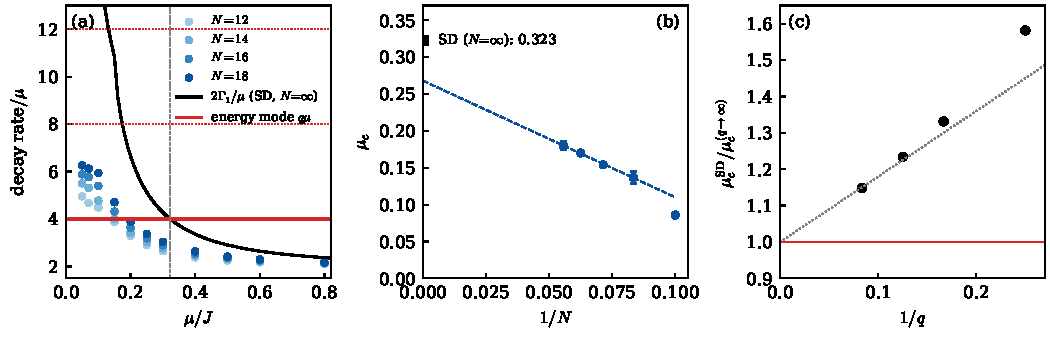
\includegraphics[width=\textwidth]{../figs/fig1.pdf}
\caption{(a) Decay rates in units of $\mu$ for $q=4$. Red line: exact energy mode $q\mu$, Eq.~\eqref{eq:exact}. Dotted lines: secular tower $kq\mu$, $k=2,3$. Dots: slowest energy-orthogonal even eigenvalue from ED, averaged over disorder ($N=12$--$18$). Black: $2\Gamma_1/\mu$ from the large-$N$ Kadanoff-Baym equation~\eqref{eq:KB}; the kink near $0.16J$ is the single-fermion exceptional point. The gap is the lower envelope of the red line and the energy-orthogonal branch; the dashed vertical line marks $\mu_c=0.323J$. (b) Crossing point $\mu_c(N)$ from ED (disorder mean $\pm$ standard error), with the linear fit for $N\ge12$ and the SD value. (c) Ratio of the SD crossing point, from $q\mu_c=2\Gamma_1(\mu_c)$, to the large-$q$ formula~\eqref{eq:muc_q}, for $q=4,6,8,12$.}
\label{fig:gap}
\end{figure*}

\emph{Gap transition.}---Combining Eqs.~\eqref{eq:gap} and \eqref{eq:gstar}, the gap at $N=\infty$ is
\begin{equation}
\Delta(\mu)=\begin{cases}q\mu, & \mu<\mu_c,\\ 2\Gamma_1(\mu),&\mu>\mu_c,\end{cases}\qquad q\mu_c=2\Gamma_1(\mu_c).
\label{eq:Delta}
\end{equation}
For $q=4$ we obtain $\mu_c=0.323J$, with $\Delta(\mu_c)=1.29J$ [Fig.~\ref{fig:gap}(a)]. At $\mu_c$ the derivative jumps from $d\Delta/d\mu=4$ to $2\Gamma_1'(\mu_c)\approx0.46$. The relaxing mode also switches character, from a size-$q$ operator (the energy) to a bilinear. In ED the crossing is exact at every $N$ [Eq.~\eqref{eq:gap}], and $\mu_c(N)$ grows monotonically from $0.086J$ at $N=10$ to $0.180J$ at $N=18$ [Fig.~\ref{fig:gap}(b)]. A linear (quadratic) extrapolation in $1/N$ over $N=12$--$18$ gives $0.27J$ ($0.28J$). The remaining difference from the SD value reflects the slow, nonlinear convergence of $\Gamma_\ast$ near $\mu_c$, which is visible in Fig.~\ref{fig:gap}(a). Note that $\mu_c$ is distinct from the exceptional point $\mu_{\rm EP}\simeq0.16J$ of the single-fermion function, where Green's-function oscillations stop~\cite{Garcia2023}.

At large $q$, with $C=\tfrac12e^{g/q}$, Eq.~\eqref{eq:KB} reduces to the Liouville equation $\ddot g=-2\J^2e^g$ with $g(0)=0$ and $\dot g(0)=-q\mu$. Its solution $e^{g}=\alpha^2/[\J\cosh(\alpha t+\gamma)]^2$ has $\alpha=\sqrt{\J^2+(q\mu/2)^2}$, so $\Gamma_1=2\alpha/q$~\cite{Kulkarni2022}. The crossing condition $q\mu_c=4\alpha/q$ then gives the closed form
\begin{equation}
\mu_c=\frac{4\J}{q\sqrt{q^2-4}}\simeq\frac{4\J}{q^2}.
\label{eq:muc_q}
\end{equation}
The full SD crossing approaches Eq.~\eqref{eq:muc_q} as $1+c/q$ with $c\approx1.8$ [Fig.~\ref{fig:gap}(c)]. In the usual large-$q$ scaling with $\hat\mu=q\mu$ held fixed, $\hat\mu>\hat\mu_c=4\J/q$, so the gap is always the energy-orthogonal resonance. The energy-mode regime appears only at the next order in $1/q$. This explains why it is absent from fixed-$\hat\mu$ large-$q$ treatments.

\emph{Energy hydrodynamics below $\mu_c$.}---For $\mu<\mu_c$ the slow sector is spanned by functions of $H$. To leading order in $\mu$, the diagonal of $\rho$ in the energy eigenbasis, $p_E$, obeys a classical master equation $\dot p_E=\mu\sum_{E'}W_{EE'}p_{E'}$ with $W_{EE'}=\sum_i|\langle E|\psi_i|E'\rangle|^2-\tfrac N2\delta_{EE'}$. Equation~\eqref{eq:exact} implies that $E$ is an exact eigenvector of $W$ with eigenvalue $-q$, and numerically it is the slowest nonstationary eigenvector for all $10\le N\le24$. The higher eigenvalues grow toward $\lambda_k=k$ [Fig.~\ref{fig:hydro}(c)]; extrapolating in $1/N$ gives $\lambda_2\approx2.0$--$2.3$ and $\lambda_3\approx3.4$, consistent with this limit within the finite-size uncertainty. This is an OU tower: the eigenfunctions are the orthogonal polynomials $P_k(H)$ of the SYK density of states, whose Majorana size is $kq[1+O(kq/N)]$. The finite-$N$ estimate $\frac N2[1-(1-2q/N)^k]$ for the size of a product of $k$ random $q$-strings reproduces the measured sizes of $P_k(H)$ to within $8\%$ for $N=20$. At large $N$ the density of states is Gaussian near $E=0$, and the OU flow maps a Gibbs state $e^{-\beta H}$ onto a Gibbs state with $\beta(t)=\beta_0e^{-q\mu t}$, because it contracts the mean while preserving the stationary width. The resulting picture is \emph{quasistatic heating}. The state tracks the instantaneous Gibbs manifold, its energy obeys Eq.~\eqref{eq:exact} exactly, and deviations from the manifold relax at the finite rate $\Gamma_\ast$. Figure~\ref{fig:hydro} confirms this by direct integration of the Lindblad equation at $N=14$ starting from Gibbs states. The trace distance to the Gibbs state of the same energy stays at about $2\%$ ($16\%$) of the distance travelled for $\beta_0J=0.5$ ($4$). The residual deviation is nearly independent of $\mu$ ($0.025$--$0.2J$ at $N=12$) and grows with $\beta_0$, consistent with the non-Gaussian finite-$N$ density of states rather than with incomplete thermalization.

\begin{figure*}[t]
\centering
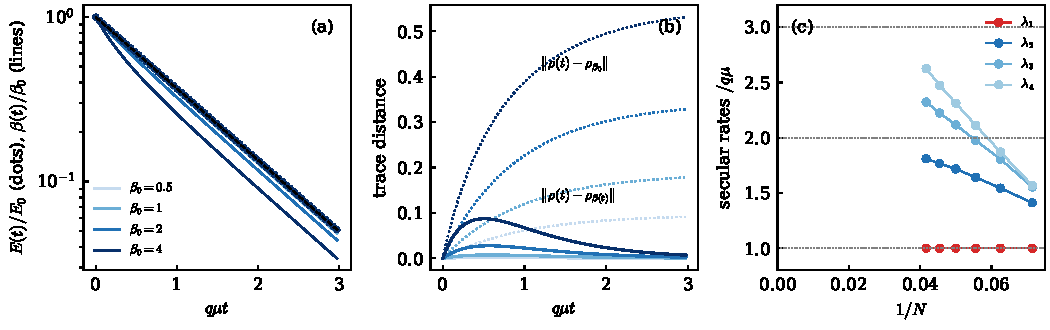
\includegraphics[width=\textwidth]{../figs/fig2.pdf}
\caption{Quasistatic heating below $\mu_c$ ($q=4$, $N=14$, $\mu=0.05J$, one realization). (a) Energy $E(t)/E_0$ (dots) follows $e^{-q\mu t}$ (dashed) exactly for every initial $\beta_0$; lines show the effective inverse temperature $\beta(t)/\beta_0$. (b) Trace distance to the instantaneous Gibbs state of equal energy (solid) compared with the distance from the initial state (dotted). (c) Secular (energy-diagonal) decay rates $\lambda_k$ in units of $q\mu$ versus $1/N$, averaged over three realizations. $\lambda_1=1$ is exact; dotted lines mark the OU values $\lambda_k=k$.}
\label{fig:hydro}
\end{figure*}

\emph{Discussion.}---Equation~\eqref{eq:Delta} answers the question posed above. The finite decay rate of the fermion Green's function in the limit $\mu\to0$~\cite{Kulkarni2022,Garcia2023} is real, but it belongs to the energy-orthogonal sector, which contains the Green's functions and every observable orthogonal to $H$. The Lindbladian gap of the physical state space closes linearly, $\Delta=q\mu$, for $\mu<\mu_c$, in agreement with Mori's general expectation for systems with a conserved quantity~\cite{Mori2024}. Here the mechanism is exact: there is no order-of-limits ambiguity, because Eq.~\eqref{eq:exact} holds at every $N$. Relaxation below $\mu_c$ is therefore two-stage. Correlations orthogonal to the Gibbs manifold decay at the anomalous rate $\Gamma_\ast\approx2\Gamma_1$, while the energy distribution drifts along an OU tower with rates $kq\mu$. This is the dissipative counterpart of the familiar separation between scrambling and hydrodynamic relaxation in closed chaotic systems~\cite{Jacoby2025,Zhang2026}. The gap transition at $\mu_c$ marks the point where the bath heats the system faster than its intrinsic resonances can keep it thermal.

In the holographic reading of Ref.~\cite{Garcia2023}, $\Gamma_\ast$ is a quasinormal decay rate of the Keldysh-wormhole geometry, and $H$ is the boundary energy, i.e., the ADM mass of the dual near-AdS$_2$ black hole. Equation~\eqref{eq:exact} then states that the bath extracts the mass at a rate independent of the geometry. The transition at $\mu_c$ separates adiabatic evolution of the black hole through a sequence of equilibrium geometries ($\mu<\mu_c$) from a regime where the mass changes faster than the ringdown. More broadly, Eq.~\eqref{eq:gap} gives a falsifiable criterion for digital or analog quantum simulations of SYK-like and spin models~\cite{Danshita2017,Jafferis2022}. With size- or weight-homogeneous Hamiltonians and uniform noise, the measured energy decay is a pure exponential at the noise-set rate, and the asymptotic relaxation of all other observables switches from this rate to an intrinsic resonance at a sharp noise strength. Natural open questions include the fate of the crossing when the grading is broken weakly, which turns it into an avoided crossing of width set by the size-inhomogeneity of $H$; the analogous construction in the double-scaled limit, where the OU tower should become a $q$-deformed OU process on the chord Hilbert space~\cite{Berkooz2019,Lin2022}; and an analytic treatment of the even-sector ladder that controls the $1/N$ corrections to Eq.~\eqref{eq:gstar}.

\emph{Numerical methods.}---ED uses Jordan-Wigner Majoranas and the block structure of even operators in the fermion-parity basis (dimension $2^{N-1}$ per sector). Leading eigenvalues on $\mathcal V_\perp$ were computed with shift-deflated Arnoldi iteration (tolerance $10^{-6}$--$10^{-8}$). For $N=12$ we cross-checked against full diagonalization. Eq.~\eqref{eq:KB} was integrated with a second-order predictor-corrector scheme ($\delta t=0.004/J$, $T=60/J$), and $z_1$ was obtained by Newton iteration on the Laplace-transformed kernel. Lindblad evolution in Fig.~\ref{fig:hydro} used fourth-order Runge-Kutta ($\delta t=0.02/J$). Code and data are available from the author.

\begin{thebibliography}{99}
\bibitem{Kessler2012} E.~M. Kessler, G. Giedke, A. Imamoglu, S.~F. Yelin, M.~D. Lukin, and J.~I. Cirac, Phys. Rev. A \textbf{86}, 012116 (2012).
\bibitem{Minganti2018} F. Minganti, A. Biella, N. Bartolo, and C. Ciuti, Phys. Rev. A \textbf{98}, 042118 (2018).
\bibitem{Znidaric2015} M. \v{Z}nidari\v{c}, Phys. Rev. E \textbf{92}, 042143 (2015).
\bibitem{Prosen2002} T. Prosen, J. Phys. A \textbf{35}, L737 (2002).
\bibitem{Mori2024} T. Mori, Phys. Rev. B \textbf{109}, 064311 (2024).
\bibitem{Jacoby2025} J.~A. Jacoby, D.~A. Huse, and S. Gopalakrishnan, Phys. Rev. B \textbf{111}, 104303 (2025).
\bibitem{Zhang2026} T. Zhang, X. Nie, and C. von Keyserlingk, Phys. Rev. Research \textbf{8}, 033186 (2026).
\bibitem{SY1993} S. Sachdev and J. Ye, Phys. Rev. Lett. \textbf{70}, 3339 (1993).
\bibitem{Kitaev2015} A. Kitaev, talks at KITP (2015).
\bibitem{MS2016} J. Maldacena and D. Stanford, Phys. Rev. D \textbf{94}, 106002 (2016).
\bibitem{Kulkarni2022} A. Kulkarni, T. Numasawa, and S. Ryu, Phys. Rev. B \textbf{106}, 075138 (2022).
\bibitem{Sa2022} L. S\'a, P. Ribeiro, and T. Prosen, Phys. Rev. Research \textbf{4}, L022068 (2022).
\bibitem{Garcia2023} A.~M. Garc\'ia-Garc\'ia, L. S\'a, J.~J.~M. Verbaarschot, and J.~P. Zheng, Phys. Rev. D \textbf{107}, 106006 (2023).
\bibitem{MQ2018} J. Maldacena and X.-L. Qi, arXiv:1804.00491.
\bibitem{Zheng2026} J.~P. Zheng, J. Dukelsky, R.~A. Molina, and A.~M. Garc\'ia-Garc\'ia, Phys. Rev. D \textbf{113}, 066018 (2026).
\bibitem{Schuster2023} T. Schuster and N.~Y. Yao, Phys. Rev. Lett. \textbf{131}, 160402 (2023).
\bibitem{Bhattacharjee2023} B. Bhattacharjee, X. Cao, P. Nandy, and T. Pathak, J. High Energy Phys. 03 (2023) 054.
\bibitem{Liu2024} C. Liu, R. Meyer, and Z.-Y. Xian, J. High Energy Phys. 08 (2024) 092.
\bibitem{Danshita2017} I. Danshita, M. Hanada, and M. Tezuka, Prog. Theor. Exp. Phys. \textbf{2017}, 083I01 (2017).
\bibitem{Jafferis2022} D. Jafferis \emph{et al.}, Nature \textbf{612}, 51 (2022).
\bibitem{Berkooz2019} M. Berkooz, M. Isachenkov, V. Narovlansky, and G. Torrents, J. High Energy Phys. 03 (2019) 079.
\bibitem{Lin2022} H.~W. Lin, J. High Energy Phys. 11 (2022) 060.
\end{thebibliography}

\end{document}
